\chapter{Results}
\label{sec:Results}

In this section the results of the cross-section calculations are presented. The results of the integral and differential cross-sections (as defined in Sec.~\ref{sec:ZeeCrossSec}) are shown together with uncertainties and theoretical predictions.

\begin{figure}
\center{
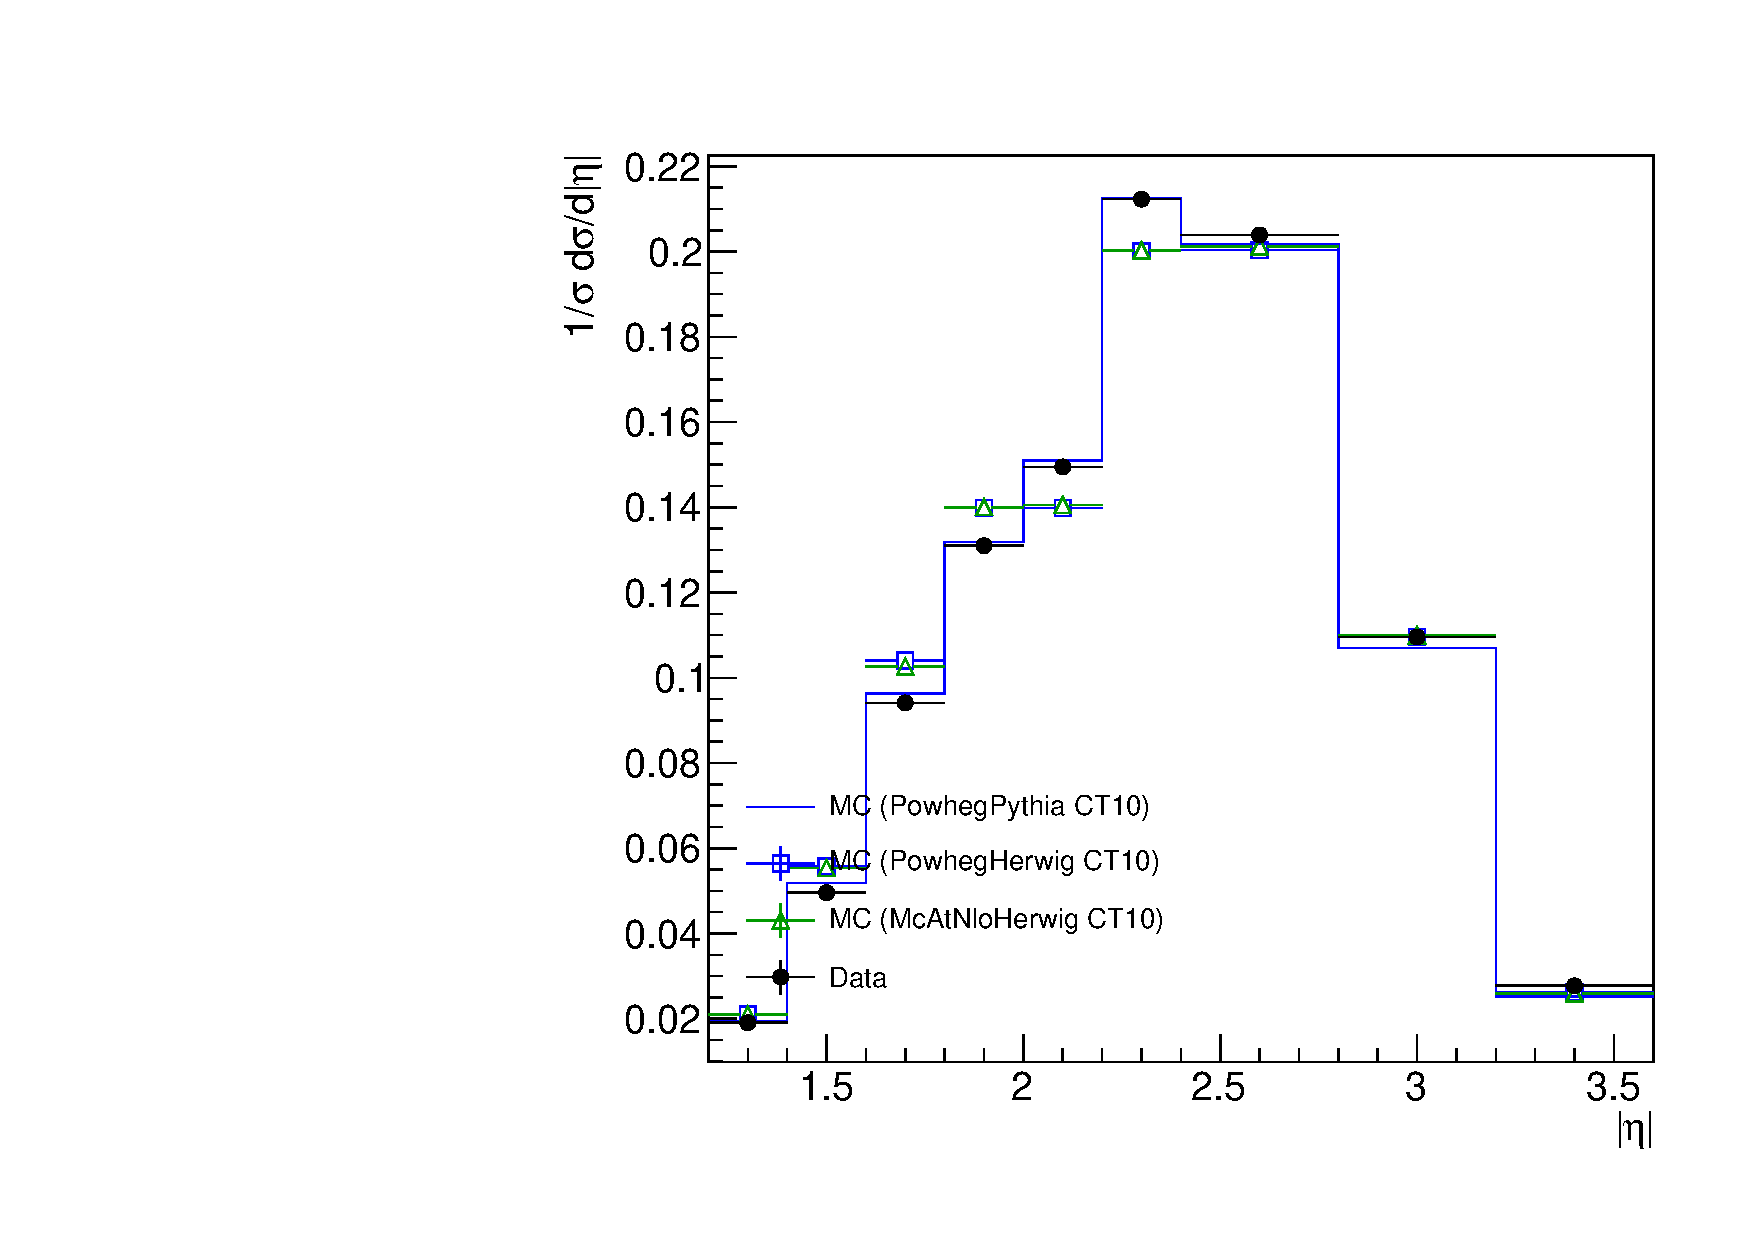
\includegraphics[width=0.45\textwidth]{figures/ZeeCF_Mass_66_116_FiduCS.pdf}
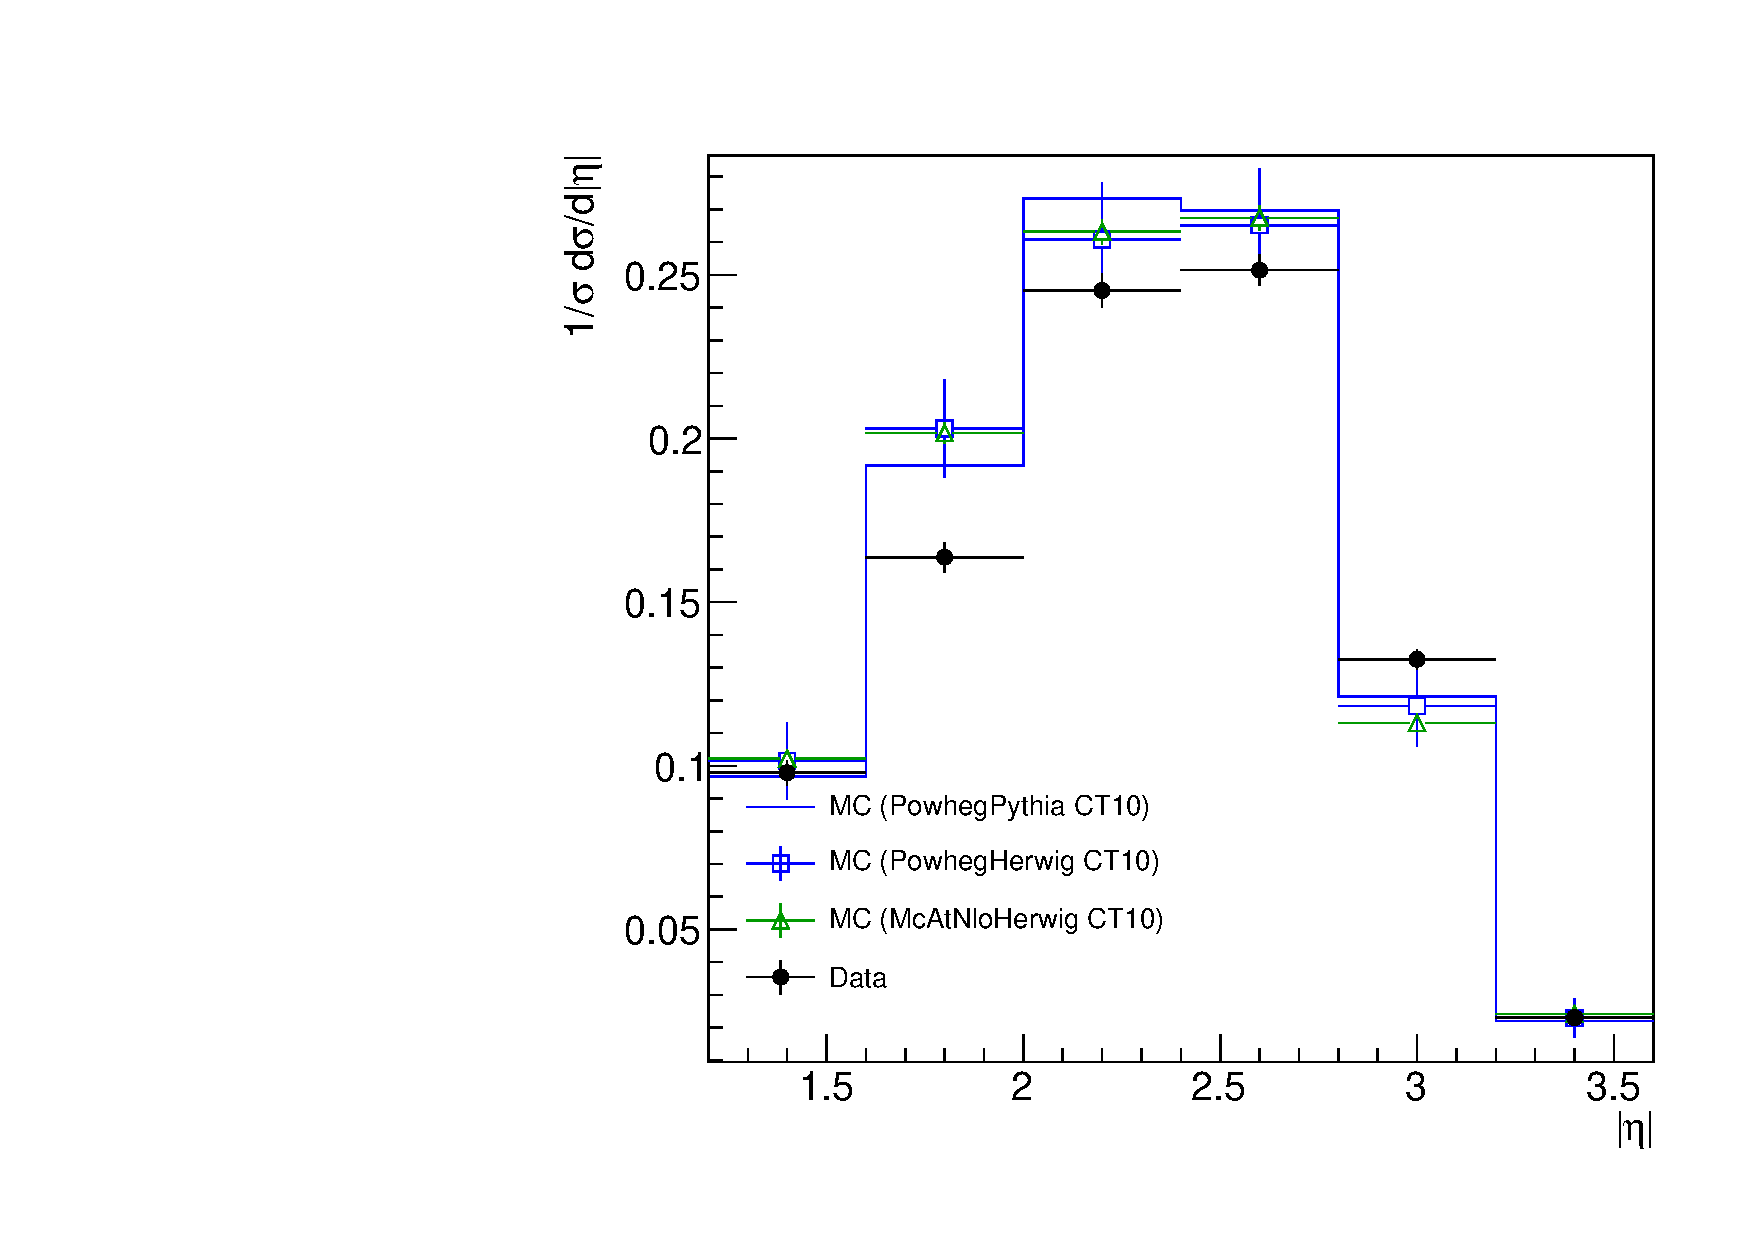
\includegraphics[width=0.45\textwidth]{figures/ZeeCF_Mass_116_150_FiduCS.pdf}
\caption{Normalised \Zee\ CF differential cross-section, as a function of absolute boson rapidity for peak mass (left) and high mass (right) regions.}
\label{fig:res_zee_fid_norm}}
\end{figure}

\begin{figure}
\center{
  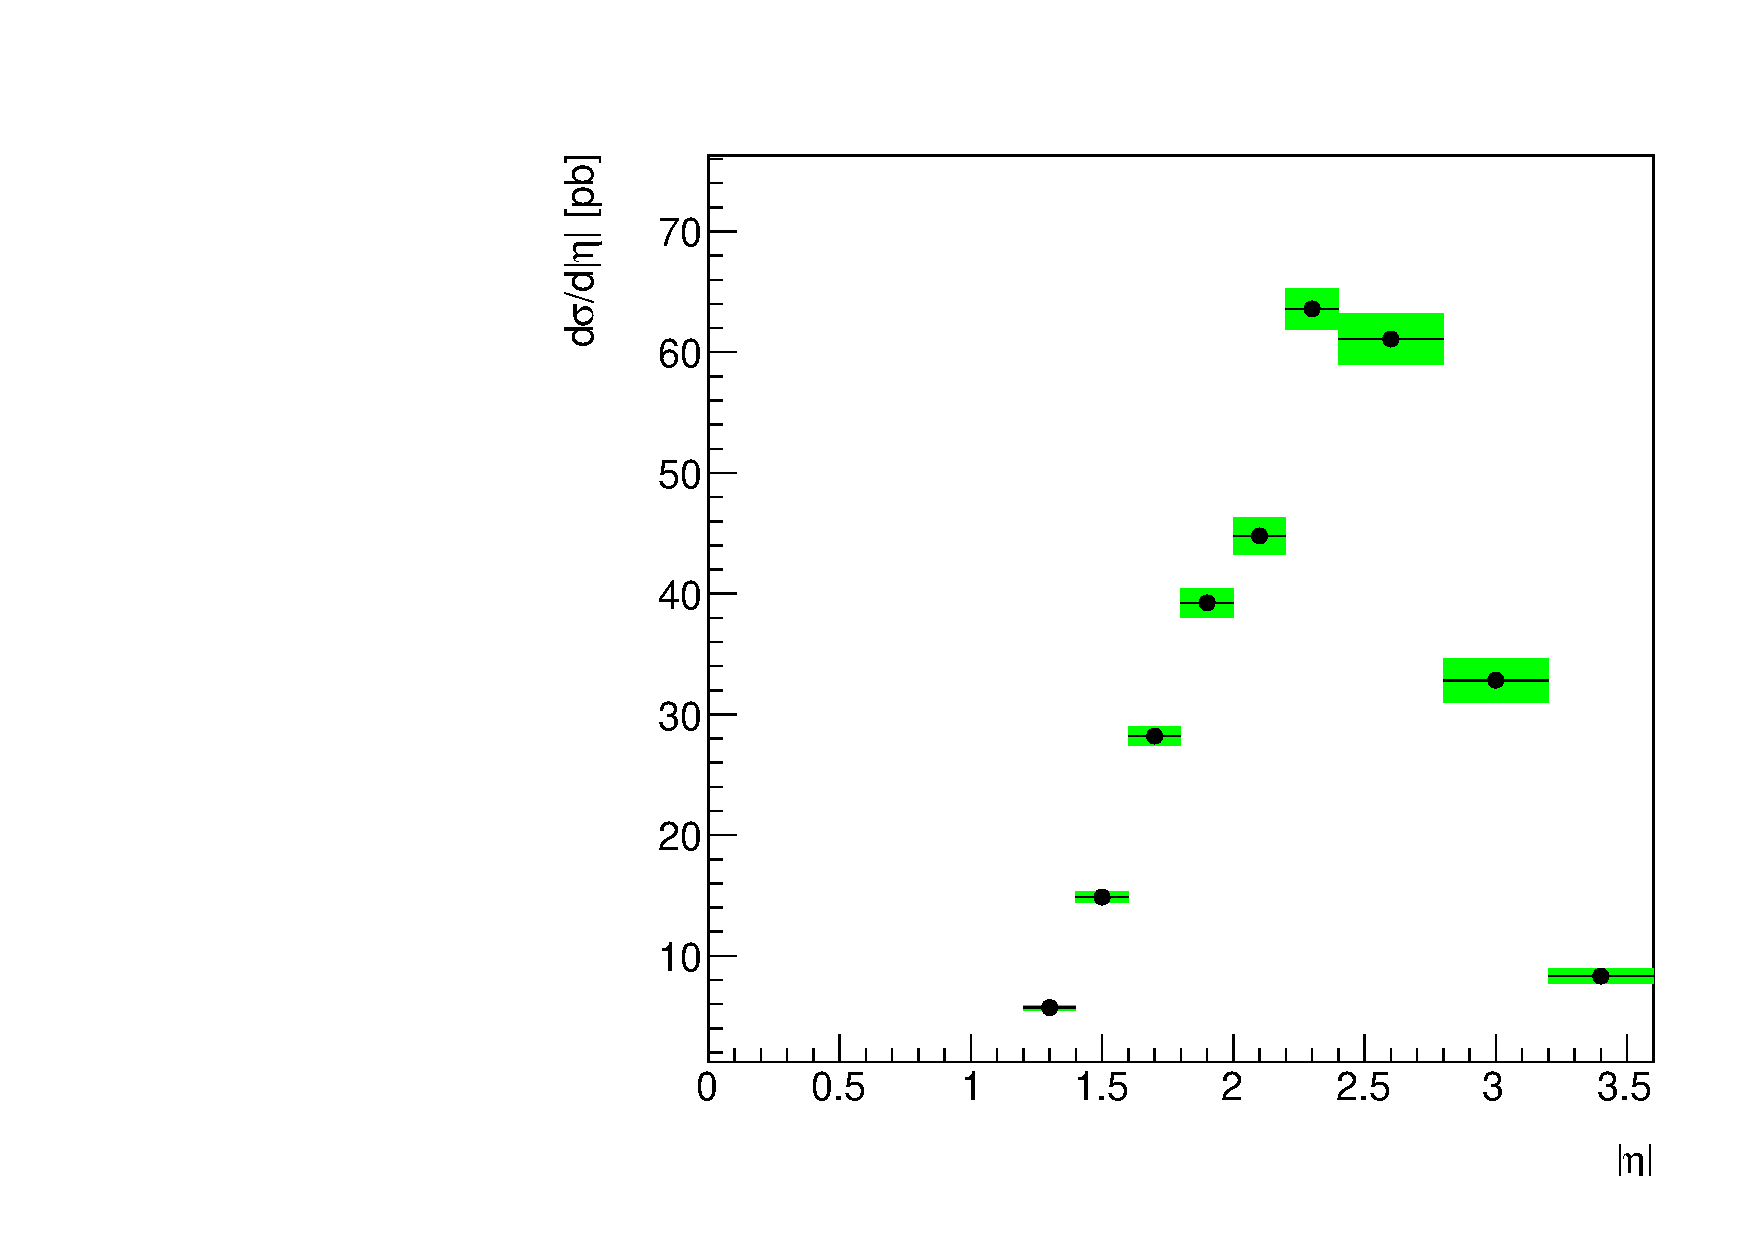
\includegraphics[width=0.45\textwidth]{figures/ZeeCF_Mass_66_116_FiduCS_band.pdf}
  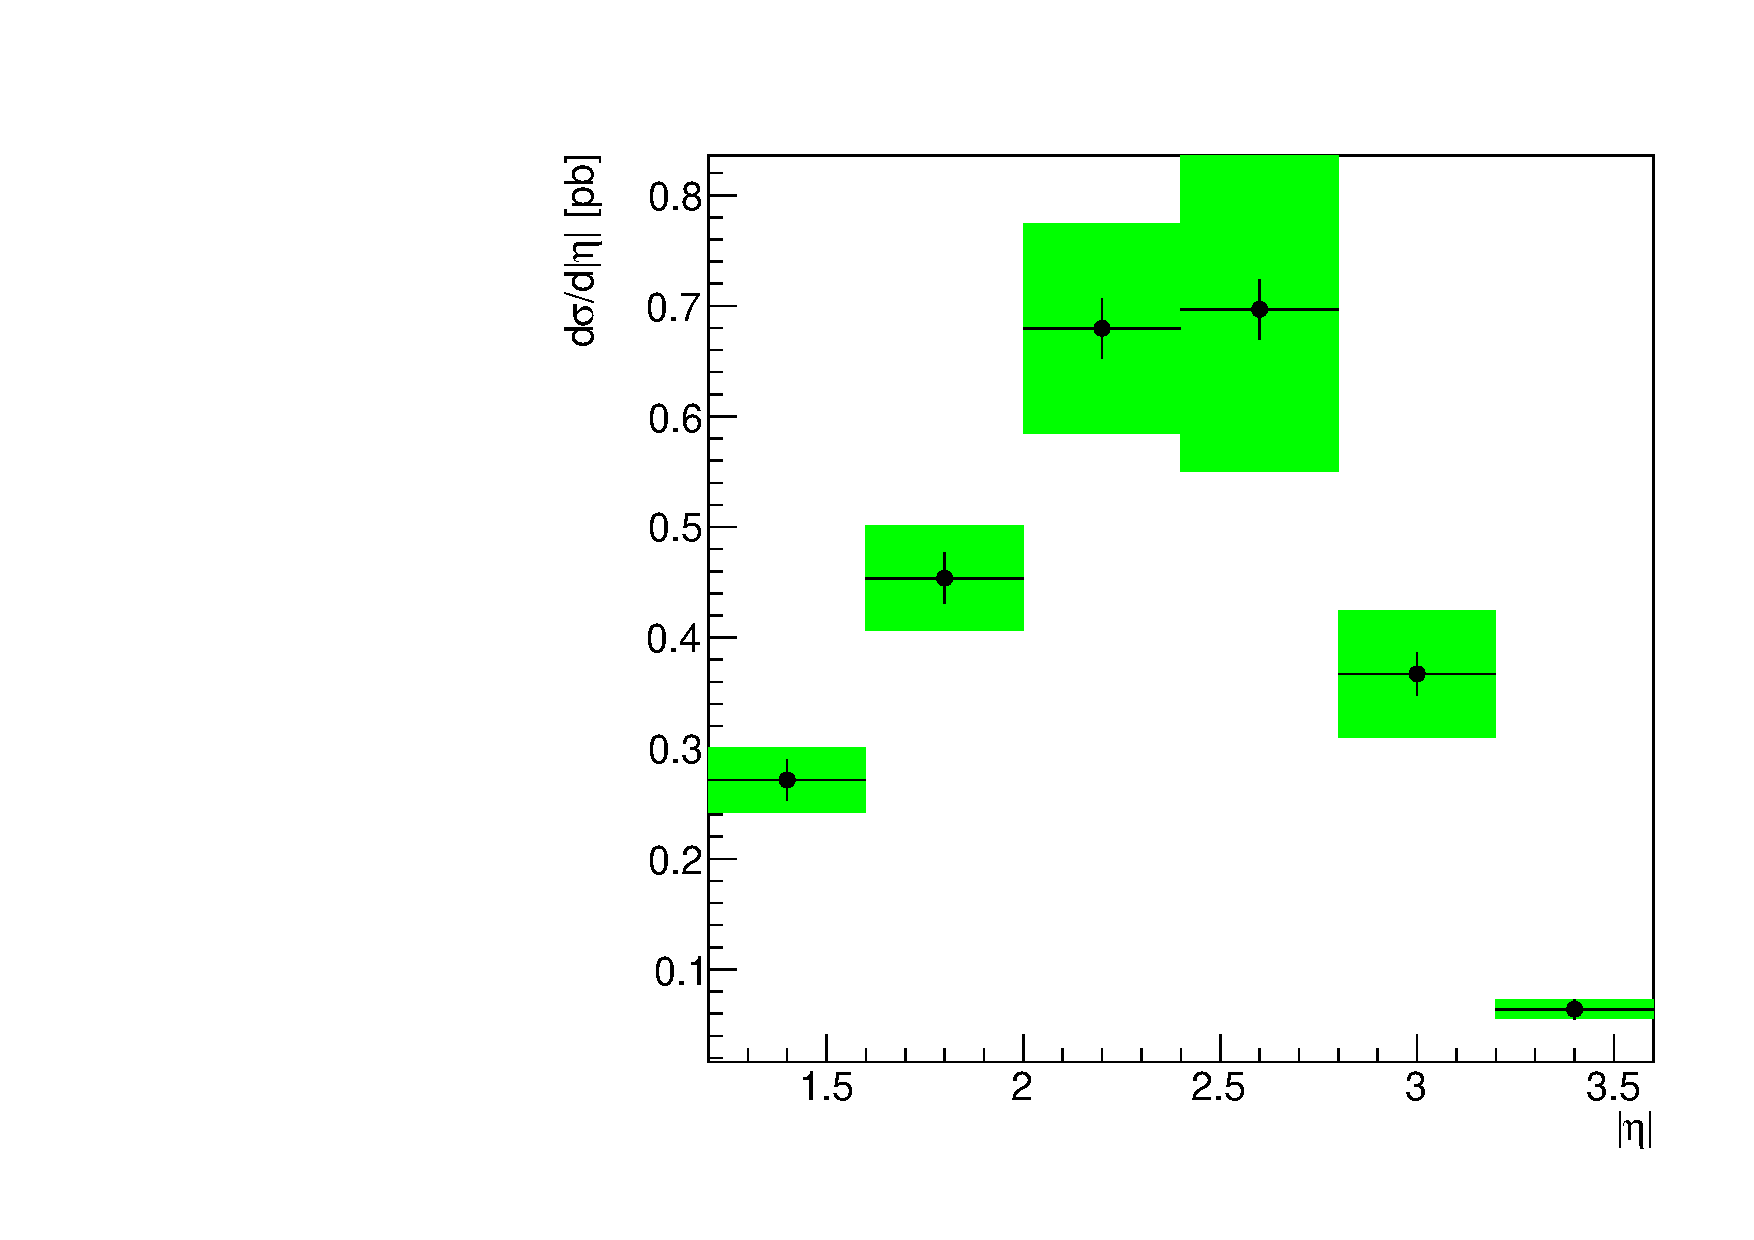
\includegraphics[width=0.45\textwidth]{figures/ZeeCF_Mass_116_150_FiduCS_band.pdf}
  \caption{\Zee\ CF fiducial diffirential cross-section, as a function of absolute boson rapidity for peak mass (left) and high mass (right) regions together with statistical and systematic uncertainties.}
\label{fig:res_zee_fid}}
\end{figure}

\begin{table}
\centering
\begin{tabular}{lccc}
\hline
    &   $N$   & $B \pm \delta B$  &  $C \pm \delta C$ \\
\hline
$\hfill 66.00 < m_{ee} <116.00$       & 321575     & 9174.1     $\pm$ 462.1 & 0.425      $\pm$ 0.010 \\
$116.00 < m_{ee} <150.00$      & 7740       & 2732.8     $\pm$ 261.8 & 0.520      $\pm$ 0.018 \\
\hline
\end{tabular}
\caption{Main components of the integrated \Zee\ CF cross-section.}
\label{tab:Zee_NBC}
\end{table}

\begin{table}
\centering
\begin{tabular}{lccc}
\hline
    &   $N$   & $B \pm \delta B$  &  $C \pm \delta C$ \\
\hline
$1.20 < |\eta| <1.40$          & 4178       & 193.7      $\pm$ 19.7 & 0.381      $\pm$ 0.014 \\
$1.40 < |\eta| <1.60$          & 12404      & 517.7      $\pm$ 47.4 & 0.436      $\pm$ 0.013 \\
$1.60 < |\eta| <1.80$          & 24210      & 812.1      $\pm$ 72.7 & 0.453      $\pm$ 0.012 \\
$1.80 < |\eta| <2.00$          & 33978      & 1021.2     $\pm$ 110.9 & 0.459      $\pm$ 0.014 \\
$2.00 < |\eta| <2.20$          & 38023      & 1141.2     $\pm$ 123.9 & 0.449      $\pm$ 0.015 \\
$2.20 < |\eta| <2.40$          & 51372      & 1454.4     $\pm$ 77.6 & 0.429      $\pm$ 0.011 \\
$2.40 < |\eta| <2.80$          & 101004     & 2613.2     $\pm$ 267.5 & 0.440      $\pm$ 0.015 \\
$2.80 < |\eta| <3.20$          & 47304      & 1104.4     $\pm$ 52.3 & 0.384      $\pm$ 0.021 \\
$3.20 < |\eta| <3.60$          & 8453       & 126.6      $\pm$ 29.5 & 0.276      $\pm$ 0.020 \\
\hline
\end{tabular}
\caption{Main components of the differential \Zee\ CF cross-section for peak mass region.}
\label{tab:Zee_NBC_peak}
\end{table}


\begin{table}
\centering
\begin{tabular}{lccc}
\hline
    &   $N$   & $B \pm \delta B$  &  $C \pm \delta C$ \\
\hline
$1.20 < |\eta| <1.60$          & 1136       & 592.4      $\pm$ 54.8 & 0.552      $\pm$ 0.024 \\
$1.60 < |\eta| <2.00$          & 1676       & 754.6      $\pm$ 79.2 & 0.565      $\pm$ 0.035 \\
$2.00 < |\eta| <2.40$          & 2006       & 737.4      $\pm$ 80.2 & 0.531      $\pm$ 0.067 \\
$2.40 < |\eta| <2.80$          & 1754       & 506.2      $\pm$ 48.6 & 0.515      $\pm$ 0.107 \\
$2.80 < |\eta| <3.20$          & 659        & 120.7      $\pm$ 12.8 & 0.439      $\pm$ 0.068 \\
$3.20 < |\eta| <3.60$          & 84         & 15.2       $\pm$ 8.3 & 0.348      $\pm$ 0.031 \\
\hline
\end{tabular}
\caption{Main components of the differential \Zee\ CF cross-section for high mass region.}
\label{tab:Zee_NBC_high}
\end{table}

\begin{table}
\centering
\begin{tabular}{lc}
\hline
$\hfill 66.00 < m_{ee} <116.00$       & 3.204 $\pm$ 0.006 (stat) $\pm$ 0.073 (syst) $\pm$ 0.058 (lum) [pb]  \\
$116.00 < m_{ee} <150.00$      & 0.063 $\pm$ 0.001 (stat) $\pm$ 0.004 (syst) $\pm$ 0.001 (lum) [pb]  \\
\hline
\end{tabular}
\caption{Integrated \Zee\ CF cross-section, measured in the experimental fiducial volume together with uncertainties.}
\label{tab:Zee}
\end{table}

\begin{table}
\centering
\begin{tabular}{lc}
\hline
$1.20 < |\eta| <1.40$          & 5.715 $\pm$ 0.101 (stat) $\pm$ 0.207 (syst) $\pm$ 0.103 (lum) [pb]  \\
$1.40 < |\eta| <1.60$          & 14.864 $\pm$ 0.151 (stat) $\pm$ 0.465 (syst) $\pm$ 0.268 (lum) [pb]  \\
$1.60 < |\eta| <1.80$          & 28.200 $\pm$ 0.206 (stat) $\pm$ 0.792 (syst) $\pm$ 0.508 (lum) [pb]  \\
$1.80 < |\eta| <2.00$          & 39.245 $\pm$ 0.233 (stat) $\pm$ 1.214 (syst) $\pm$ 0.706 (lum) [pb]  \\
$2.00 < |\eta| <2.20$          & 44.786 $\pm$ 0.260 (stat) $\pm$ 1.534 (syst) $\pm$ 0.806 (lum) [pb]  \\
$2.20 < |\eta| <2.40$          & 63.598 $\pm$ 0.317 (stat) $\pm$ 1.717 (syst) $\pm$ 1.145 (lum) [pb]  \\
$2.40 < |\eta| <2.80$          & 61.087 $\pm$ 0.207 (stat) $\pm$ 2.126 (syst) $\pm$ 1.100 (lum) [pb]  \\
$2.80 < |\eta| <3.20$          & 32.826 $\pm$ 0.162 (stat) $\pm$ 1.811 (syst) $\pm$ 0.591 (lum) [pb]  \\
$3.20 < |\eta| <3.60$          & 8.313 $\pm$ 0.102 (stat) $\pm$ 0.614 (syst) $\pm$ 0.150 (lum) [pb]  \\
\hline
\end{tabular}
\caption{Differential \Zee\ CF cross-section for the peak mass region, measured in the experimental fiducial volume together with uncertainties.}
\label{tab:Zee_peak}
\end{table}

\begin{table}
\centering
\begin{tabular}{lc}
\hline
$1.20 < |\eta| <1.60$          & 0.271 $\pm$ 0.018 (stat) $\pm$ 0.030 (syst) $\pm$ 0.005 (lum) [pb]  \\
$1.60 < |\eta| <2.00$          & 0.454 $\pm$ 0.023 (stat) $\pm$ 0.047 (syst) $\pm$ 0.008 (lum) [pb]  \\
$2.00 < |\eta| <2.40$          & 0.680 $\pm$ 0.027 (stat) $\pm$ 0.095 (syst) $\pm$ 0.012 (lum) [pb]  \\
$2.40 < |\eta| <2.80$          & 0.697 $\pm$ 0.027 (stat) $\pm$ 0.147 (syst) $\pm$ 0.013 (lum) [pb]  \\
$2.80 < |\eta| <3.20$          & 0.367 $\pm$ 0.019 (stat) $\pm$ 0.057 (syst) $\pm$ 0.007 (lum) [pb]  \\
$3.20 < |\eta| <3.60$          & 0.064 $\pm$ 0.009 (stat) $\pm$ 0.009 (syst) $\pm$ 0.001 (lum) [pb]  \\
\hline
\end{tabular}
\caption{Differential \Zee\ CF cross-section for the high mass region, measured in the experimental fiducial volume together with uncertainties.}
\label{tab:Zee_high}
\end{table}
